% THIS IS SIGPROC-SP.TEX - VERSION 3.1
% WORKS WITH V3.2SP OF ACM_PROC_ARTICLE-SP.CLS
% APRIL 2009
%
% It is an example file showing how to use the 'acm_proc_article-sp.cls' V3.2SP
% LaTeX2e document class file for Conference Proceedings submissions.
% ----------------------------------------------------------------------------------------------------------------
% This .tex file (and associated .cls V3.2SP) *DOES NOT* produce:
%       1) The Permission Statement
%       2) The Conference (location) Info information
%       3) The Copyright Line with ACM data
%       4) Page numbering
% ---------------------------------------------------------------------------------------------------------------
% It is an example which *does* use the .bib file (from which the .bbl file
% is produced).
% REMEMBER HOWEVER: After having produced the .bbl file,
% and prior to final submission,
% you need to 'insert'  your .bbl file into your source .tex file so as to provide
% ONE 'self-contained' source file.
%
% Questions regarding SIGS should be sent to
% Adrienne Griscti ---> griscti@acm.org
%
% Questions/suggestions regarding the guidelines, .tex and .cls files, etc. to
% Gerald Murray ---> murray@hq.acm.org
%
% For tracking purposes - this is V3.1SP - APRIL 2009

\documentclass{acm_proc_article-sp}

\begin{document}

\title{Renewable and Cooling Aware Geographical Load Balancing\titlenote{This research is supported by the NSF, Mr. David C. Elliot's family, and the Rose Hills Foundation.}}
\numberofauthors{4} 
\author{
% You can go ahead and credit any number of authors here,
% e.g. one 'row of three' or two rows (consisting of one row of three
% and a second row of one, two or three).
%
% The command \alignauthor (no curly braces needed) should
% precede each author name, affiliation/snail-mail address and
% e-mail address. Additionally, tag each line of
% affiliation/address with \affaddr, and tag the
% e-mail address with \email.
%
% 1st. author
\alignauthor
Michael Hirshleifer\\
       \affaddr{California Institute of Technology}\\
       \affaddr{1200 E California Blvd}\\
       \affaddr{Pasadena, California}\\
       \email{111mth@caltech.edu}
% 2nd. author
\alignauthor
Yizhen Wang\\
       \affaddr{California Institute of Technology}\\
       \affaddr{1200 E California Blvd}\\
       \affaddr{Pasadena, California}\\
       \email{ywang3@caltech.edu}
% 3rd. author
\alignauthor
Zhenhua Liu\\
       \affaddr{California Institute of Technology}\\
       \affaddr{1200 E California Blvd}\\
       \affaddr{Pasadena, California}\\
       \email{zliu2@caltech.edu}
% the prof
\and
\alignauthor
Adam Wierman\\
       \affaddr{California Institute of Technology}\\
       \affaddr{1200 E California Blvd}\\
       \affaddr{Pasadena, California}\\
       \email{adamw@caltech.edu}
}

\date{27 August 2012}

\maketitle
\begin{abstract}
This paper explores how geographical load balancing can improve the efficiency of renewable energy use in data centers.
The model incorporates the varying cooling efficiency (considering weather conditions) and electricity prices over time at each data center.
We run a convex optimization using as input real workload, temperature, solar, and wind traces.
We find that using geographical load balancing lets data centers more effectively use locally available renewable energy, thereby substantially reducing their usage of grid electricity. This conclusion holds across seasons.
We develop a visualization that displays the demand from each of the 48 contiguous U.S. states and the energy usage, grid energy usage, and renewable energy generation at each of 10 data centers, animated over time according to the input data and the optimization output. The resulting software can be used to test effectiveness of and refine routing algorithms.


\end{abstract}

\section{Introduction}


\subsection{The problem}
	\subsubsection{Energy cost is important for DCs.}
		Building cost-saving and environmentally friendly data centers has become a pressing challenge for the ICT industry.
		Energy consumption accounts for much of a data center’s running cost \cite{datacenter}, and the carbon dioxide emissions consequent to data centers’ grid energy usage concerns society at large.
		As the need for data centers grows rapidly,
		“Green” routing algorithms would benefit Internet companies by reducing their electricity costs, and everyone else by reducing pollution from non-renewable energy. The social benefit could be substantial, as data centers are expected to use several percent of U.S. and world electricity output, and they currently use mostly non-renewable energy.
		
		\paragraph{Servers use energy to process requests}
			Data centers require a substantial amount of energy, varying with load (requests processed per second).
		\paragraph{Energy usage for cooling also matters}
			
			The previous GLB model only considers the energy cost of running the servers. But in reality, a data center spends a considerable amount of energy on cooling \cite{datacenter}, especially in summer. The energy needed for cooling largely depends on the weather at data center locations. Thus we can also exploit the geographical heterogeneity of the data centers to reduce cooling cost.
	\subsubsection{Need for load balancing between DCs}
		There are often several redundant data centers, each of which can process a user request, such as a Google search. Traditionally, a request would be routed to the geographically-nearest data center, thereby minimizing latency.
	\subsubsection{Load, energy availability, grid electricity prices, etc. are time-varying and stochastic.}
		\paragraph{Renewable vs. grid energy}
			Currently, data centers are powered mainly by buying electricity off the grid. Grid electricity necessarily comes substantially from burning fossil fuels, because with current technology, storing renewable energy over time to match demand is prohibitively expensive.
			
			However, some data centers are already partly operated on green energy. Data centers may have dedicated renewable energy generation (solar or wind farms). But the renewable power output at each location varies over time (time of day, cloud cover, wind speed), and generally does not match user demand, so excess demand must be satisfied by buying electricity off the grid.


\subsection{Previous work}
	\subsubsection{Geographical load balancing}
		Geographical load balancing provides goody gooder stuff.
		Flexibility in routing could allow a network of data centers to run almost entirely off renewable energy. When routing a request, there is a trade-off: instead of always choosing the nearest data center, a request can be routed to a data center where renewable energy is currently being produced (reducing electricity costs), at the expense of somewhat higher latency. Professor Wierman’s group have devised optimal or near-optimal (given a functional form for the business cost of increased latency) routing algorithms for efficient geographical load balancing.
		\paragraph{Can use almost entirely renewables}
			Previous research suggests that the data center can even operate almost entirely on renewable energy under the geographical load balancing (GLB) model \cite{adam:GLB}. 
		\paragraph{Convex optimization framework; solve numerically}




This paper illustrates that a new geographical load balancing model which considers energy cost in cooling is able to reduce the total cost significantly compared to previous models. This improvement in green energy usage leads to much lower carbon emissions.

We set up an experiment to investigate the economic and environmental impact of our new model. We use real traces of data center workload, renewable energy availability and weather to numerically compute the optimal solution. The cost model of the geographical load balancing system is analytically determined@@@@[what that mean lah].

Our study leads to three major findings.

First, the new GLB model, the Cooling-aware GLB model, reduces the total cost of the system. This is because it is able to distribute the request to locations with not only cheap energy, but also favorable weather for cooling, thus achieves the overall optimal result. More excitingly, the optimal cost does not vary much with seasonality. This can potentially solve the problem of data center cooling in place with extreme weather, for example large day and night temperature difference.  

Second, the Cooling-aware GLB model leads to significant carbon emission savings. The carbon emission level can be reduced by as much as more than 50\% compared to the old models. The new GLB model makes more informed decision than the old GLB model as it includes the energy for cooling. Because GLB models reduces energy cost at the expense of slight increase in network delay cost, the environmental impact is much greater than the cost impact. If the firms are given incentives for cutting carbon emission, the environmental impact can lead to economic success.  

Third, the performance of Cooling-aware GLB is better than using energy storage, both in total cost and in carbon emission, when the aggregate renewable supply is enough to power data centers yet not in vast surplus. This result is from a systematic comparison between the Cooling-aware GLB system and the storage system with various storage capacity in reasonable range. The result suggests that Cooling-aware GLB has a clear advantage over the storage model when the renewable energy generation and storage facilities are not widely established. It requires much less investment in infrastructure and hence can be implemented more easily than the storage model.


\subsection{More details on the visualization blahblablablablablablablablahhh}
@@@@@@@

\subsubsection{Objectives}
Build a computer simulation of the whole data center routing system, that can use real-world data on wind and solar power output, grid electricity prices, and Internet request volume over time at various locations. Devise and implement comprehensible visualizations of the multi-dimensional simulation data. The resulting software can be used to test effectiveness of and refine routing algorithms.

The software can then be used to answer questions about extensions to the model that would be useful when putting it into practice, such as—
\begin{itemize}
\item incorporating other kinds of renewables into the model
\item no longer treating data centers as static. In the long run, where should we build new data centers, and what local renewables and energy storage systems do we use?
\item finding the optimal control timescale. It is costly to switch on and off servers, so the current algorithms only change routing every fixed period, which is suboptimal. This significantly restricts the savings that follow-the-renewables routing can yield, but the topic hasn’t yet been explored deeply. Obviously being able to simulate the whole system helps for this.
\item helping discover and then exploit emergent phenomena when looking at systems of many data centers. An example of such a phenomenon deals with the optimal mix of renewable energy for powering data centers. Since the sun shines in the daytime when people are awake and searching the Internet, one might expect solar power to dominate. But Wierman’s paper showed that in fact wind is more effective, because its low spatial and temporal correlation is especially useful for geographical load balancing. With solar power, when requests come at night you are forced to buy electricity off the grid, but with wind power, it’s almost always windy somewhere.
\end{itemize}

\subsubsection{Work plan @@@@@@@@@@@}


I wrote a Scala script to generate an animated SVG map according to input data


The script reads in and displays data center locations, client (request source) locations, and real solar- and wind-generation traces.

@@@@includes the output of the Matlab scripts (that is, the routings optimized according to the various algorithms

It was tested and verified to work in Firefox, Chromium, and the W3C SVG validator.


\item We also intend to create a wrapper web page to make the simulation easier to use, by letting users zoom into, pan, play, pause, and seek into the animation. We may also include other features like showing/hiding types of map elements.


Remaining tasks:
\begin{itemize}
\item Consider what variations in the algorithms and model are worth exploring.
\item Use the software to explore variations in the algorithms, and their performance under variations of the model.
\end{itemize}

\subsubsection{Measure of success}
A successful result will consist of simulation and visualization software that can evaluate the performance of routing algorithms, under conditions defined by actual data on data center placement, renewable power output over time and location, workload over time, etc.. The software will help develop the end goal of an implementable algorithm / system for routing Internet requests that allows data centers to operate using almost exclusively renewable energy.



\section{Setup}
We assume that each data center has a cooling system described in \cite{adam:cooling}, and then modify the model in \cite{adam:GLB} to include energy cost of cooling. The model can be solved using convex optimization technique as proved in \cite{adam:GLBfull}.
\subsection{The workload}
Let $J$ be the set of sources of requests. Each continental state in US has a source of request located at its geographical center. We quantify the amount of request by $L_j(t)$, the mean arrival rate from source $j \in J$ at time interval $t$. $L_j(t)$ is estimated using real-world traces. The base trend of the workload is taken from a trace at Hewlett-Packard Labs, then the workload of each request source is scaled proportionately to the population of the state, following by a shift along the time dimension according to the timezone.

    
\subsection{The availability of renewable energy}
We have three major considerations when modeling the availability of renewable energy:  

First, the weather at the data centers is crucial as it determines the renewable energy output per plant unit. We use real traces of wind speed and solar irradiance obtained from \cite{renew1} \cite{renew2} @@@@@@[Is this true? I thought the traces were (calculated) power output.]. The measurements have a granularity of 10 minute. The rate of renewable energy generation per plant unit at each data center is then set to be proportional to the weather data respectively.

Second, the size of the renewable energy plant matters. We scale the renewable generation capacity such that the total renewable energy is $c$ times as much as the total energy demand to process all requests. In our experiment, $c$ varies in [0.5, 4] with step length of 0.5.  

Third, we need to find the optimal ratio of solar and wind energy to power the data centers. Previous research \cite{adam:GLB} suggests that a mix of 80\% of wind and 20\% of solar fits the data center energy consumption characteristics nicely. We adopt this ratio in our experiment throughout.

\subsection{The internet-scale system}
The internet-scale system consists of a set $N$ of 10 data centers at the Google data center locations in the following states: California, Washington, Oregon, Illinois, Georgia, Virginia, Texas, Florida, North Carolina, and South Carolina. The number of servers $X_i$ at data center $i$ is set to be twice as much as the peak load at $i$ if all requests are routed to the nearest data centers.

The optimization will determine the routing plan $\lambda_{ij}(t)$ and the number of active servers $x_i(t)$ that minimizes the total cost (the sum of delay cost, energy cost, and switching cost).

\subsubsection{Delay cost}
The delay cost represents the lost of revenue incurred due to the delay in processing requests. It comprises the propagation delay $d_{ij}$ from source $j$ to date center $i$ and the queuing delay at $i$.
The propagation delay $d_{ij}$ is calculated to be the time needed to travel between $i$ and $j$ at transmission speed of 200km/ms@@@@fmt plus a constant term 5ms. The queuing delay is calculated from the parallel M/G/1/Processor Sharing queue model in which the total load $\lambda_i(t)=\sum_j \lambda_{ij}(t)$ is distributed evenly across $x_i(t)$ homogeneous servers of service rate \mbox{$\mu_i$ = $0.1(ms)^{-1}$}.

\subsubsection{Cooling optimization}
The cooling optimization model finds the minimum energy consumption required to maintain the data center at constant temperature $T = 25^{\circ}C@@@@@fmt$. A typical data center uses both air cooling and chilled water cooling. Let $x = x_a + x_c$ be the total number of active servers, $x_a$ be the number of those cooled by air cooling and $x_c$ cooled by chilled water. This model finds the best division between $x_a$ and $x_c$. 

Quantitatively, the energy consumption of air cooling is given by 
\begin{equation}
c_a(x) = kx^3, 0 \leq x \leq \bar{x}, k > 0
\end{equation}
The parameter $k$ is proportional to the temperature gradient between the inside and outside air. The $\bar{x}$ corresponds to the maximum number of the servers that can be cooled by air cooling alone. The cap $\bar{x}$ is proportional to both the temperature gradient and the maximum air flow rate. In our experiment, the air flow rate is set such that when the outside temperature is $20^{\circ}C$ lower than $T$, the data center can rely on air cooling entirely at full workload.

The energy consumption of chilled water cooling, on the other hand, is almost linear to the IT demand empirically, i.e.,
\begin{equation}
c_c(x) = \gamma x
\end{equation}
%Here $\gamma = 0.17$, meaning that the chiller takes 0.17kW/h electricity to cool the heat caused by 1kw/h of IT demand.

The optimal cooling portfolio can be written as follows:
\begin{equation}
c(x) =  \min_{x_c \in [0,x]} \gamma(x-x_c)^+ + kx_2^3
\end{equation}
which yields
$$
c(x) = \left\{ \begin{array}{ll}
         kx^3 & \mbox{if $x \geq x_s$}\\
        kx_s^3 + \gamma (x-x_s) & \mbox{otherwise}\end{array} \right.
$$
where $x_s = \min \left\{\sqrt{\gamma/3k}, \bar{x}\right\}$ is the threshold when chiller cooling is necessary.

To explore the impact of seasonality on the performance of the cooling model, we use two sets of temperature data. One is taken from the first week of January 2012 from \cite{temp}; the other is take from the first week of July 2012. The measurements are taken hourly.

\begin{figure*}
\centering
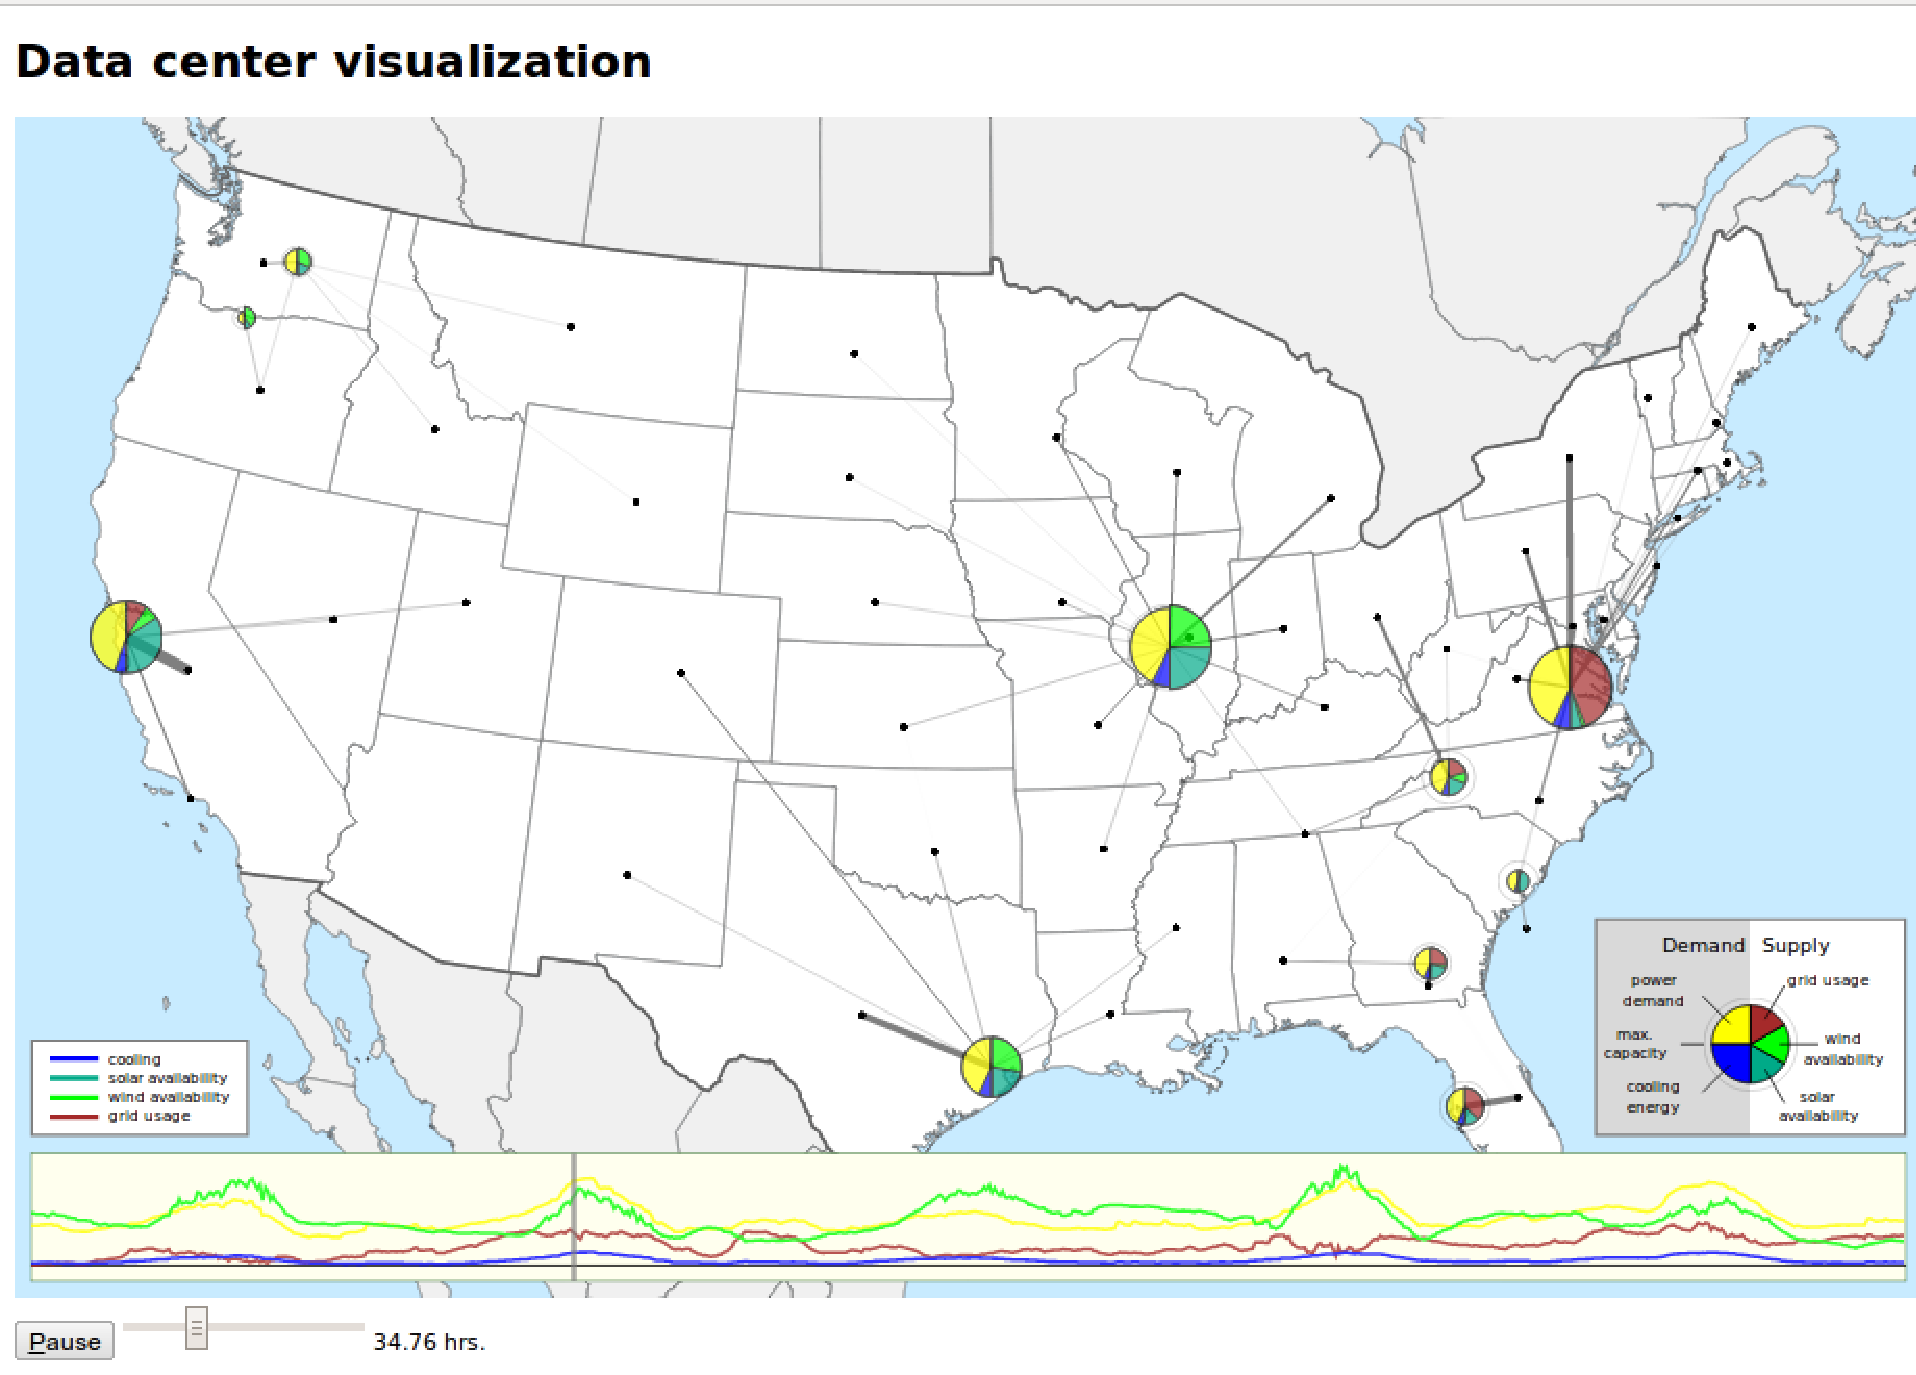
\epsfig{file=visualization-bmp.pdf, height=3in, width=4.5in}
\caption{Screenshot of the visualization, running in the Chromium web browser.}
\end{figure*}
\subsubsection{Energy cost}
The energy cost is the cost of both running active servers and keeping them at constant working temperature. The data centers pay no cost for renewable energy assuming that each data center has its own renewable energy generation facilities and pay no maintenance cost. Thus the energy cost is for using energy from the grid and can be represented as
\begin{equation}
p_i(l(x_i(t)) + c(x_i(t)) - r_i(t))^+
\end{equation}  
where $p_i$ is the price of electricity, $x_i(t)$ is the number of active servers at that time interval $t$, $l(x_i(t))$ is energy consumption of active servers in the time interval, or the IT demand, $c(x_i(t))$ is the energy usage for cooling and $r_i(t)$ is the renewable energy availability. In our model, $p_i$ is set to be constant according to the real statistics of each state; $l$ is a linear function of $x(t)$.

\subsubsection{Switching cost}
The switching cost models the delay and wear-and-tear cost when switching on/off servers. In our model, the workload at each data center is updated every 10 minutes. To avoid too frequent switching of server status, we define the switching cost to be
$$\beta(x_i(t+1) - x_i(t))^+$$
where $\beta$ tells the weight of switching cost. In our experiment, $\beta = 6$.

\subsubsection{Storage}
Apart from the renewable energy generation facility, the data centers may also install storage capacity. The renewable energy availability displays significant temporal variation; introducing storage aims to obtain soother renewable supply curve.

Quantitatively, we model the amount of electricity storage at time $t$ to be $0 \leq es_i(t) \leq ES_i$, where $ES_i$ is the maximum storage capacity. Let the amount of change of storage be 
$$e_i(t) = \rho (es_i(t) - es_i(t+1))$$
Positive $e_i(t)$ means discharging while negative value means charging. The parameter $\rho$ represents the charging and discharging efficiency. In our experiment we assume perfect charging and discharging, i.e. $\rho = 1$.

In the presence of storage capacity, the energy cost should be written as 
\begin{equation}
p_i(l(x_i(t)) + c(x_i(t)) - r_i(t) - e_i(t))^+
\end{equation} 

\subsubsection{Total cost}
Now we can formally write our optimization problem as:
\begin{align*}
\min_{\bf{x}(t), \bf{\lambda}(t)} & \sum_{i \in \mathcal{N}} p_i(l(x_i(t)) + c(x_i(t)) - r_i(t) - e_i(t))^+ \\
& + \sum_{j \in \mathcal{J}}\sum_{i \in \mathcal{N}}
\lambda_{ij}(t)\left(\frac{1}{\mu_i - \lambda_i(t)/x_i(t)} + d_{ij}\right) \\
& + \beta(x_i(t+1) - x_i(t))^+
\end{align*}
subject to
\begin{align*}
& \sum_{i\in \mathcal{N}}\lambda_{ij}(t) = L_j(t), &\forall j\in J  \\
& \lambda_{ij} \geq 0, & \forall i\in N, j\in J  \\
& 0 \leq x_i(t) \leq X_i, & \forall i \in N  \\
& \lambda_i(t) \leq x_i(t)\mu_i & \forall i \in N \\
& 0 \leq es_i(t) \leq ES_i & \forall i \in N \\
& e_i(t) = es_i(t) - es_i(t+1) & \forall i \in N
\end{align*}

The boundary conditions essentially model the following real world constraints:
\begin{enumerate}
\item
The requests from a population center all have to be processed by the geographical load balancing system. Each data center should receive a non-negative amount of work.
\item
Each data center has only limited number of servers; it cannot process requests more than its computation capacity at any time.
\item
Each data center also has limited energy storage capacity; it cannot store any amount of energy more than that cap.
\end{enumerate}
\subsubsection{CO2 emission}
Though the optimization is completely based on firm's interest of cost saving, we still want to monitor the amount of CO2 emission as a worth-noting side-effect. The CO2 emission arises from the grid electricity usage. The CO2 emission rate per kW/h varies across different states as each state has different energy source composition. An estimation of the rate can be found at \cite{carbon}.

Let $\eta_i$ be the rate of carbon emission per kW/h at data center $i$, the total CO2 emission is then
$$\sum_{i \in \mathcal{N}} \eta_i(x_i(t) + c(x_i(t)) - r_i(t) - e_i(t))^+$$ 
\subsubsection{Benchmarks for comparison}
Our model is the first to integrate practical cooling concerns into geographical load balancing. To show the impact of such consideration, we will compare the result of our model (Cooling-aware GLB) to the old GLB model which doesn't take cooling in the optimization (Cooling-Oblivious GLB) and the model which simply routes all requests to the nearest data centers (LOCAL). For the two benchmark models, the cooling optimization is done after the routing scheme is determined.

Meanwhile, we want to compare the performance of our model to one of its alternative, the storage model. The storage capacity is quantified in terms of the time period that the data center can operate entirely on storage at maximum load (excluding cooling requirement). We assume that the storage incurs no running cost. We choose the data center systems with 3-hour-storage and 6-hour-storage respectively as the benchmark. 

We will evaluate the results based on 1) the total cost; 2) the grid (brown) energy usage; 3) the $CO_2$ emission.


\begin{figure*}
\centering
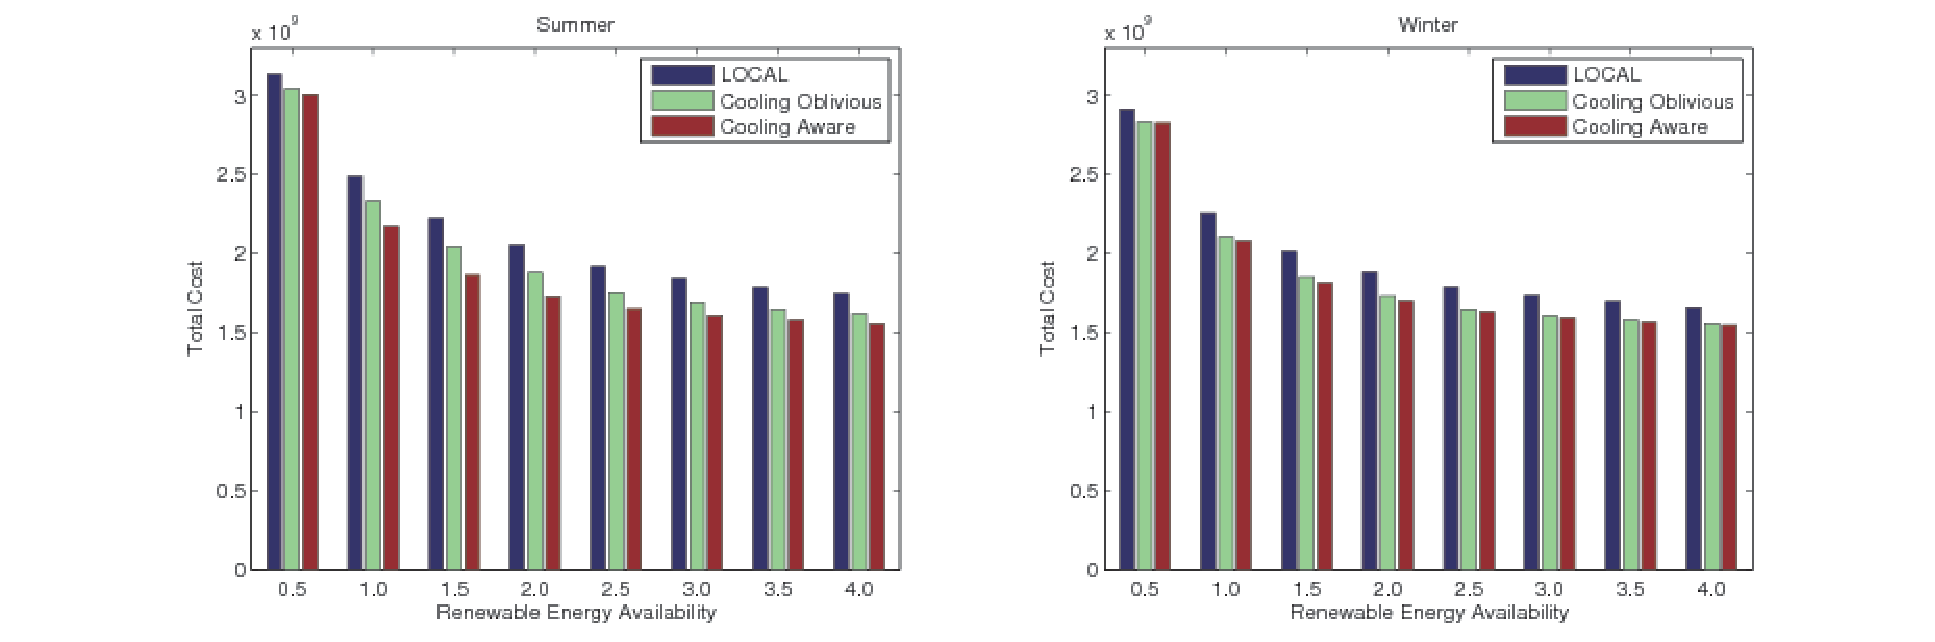
\epsfig{file=cost_comparison.pdf, height=1.8in, width=7in}
\caption{Comparison of optimal costs of Cooling-aware GLB, Cooling-oblivious GLB and LOCAL, with varying renewable energy availability.}
\end{figure*}
\section{Visualization}
Our numerical experiment often yields large size of time series data that describes routing plans and data center running status. These data are hard to interpret when in matrix form. Therefore we developed an visualization tool to illustrate these data. Such data visualization allows us to recognize the key characteristics of the optimal solution quickly. It also works as a simple check for the correctness of the solution; we can spot some obviously abnormal behaviors of the solution if they exist. 


\subsection{Development environment}
We want our visualization to satisfy the following requirement. First, it can animate a time series of data fluently. Second, it can easily and efficiently convert the raw input, usually the experiment result in .csv or .netCDF format, to the desired format recognized by the script. Third, it can be integrated into web page or other form of presentation easily. 

The final visualization is in Scalable Vector Graphics (SVG) format, a high-quality XML-based vector graphics format supporting various animations and flexible edition@@@@@@@. The back-end processing, which involves converting input file format and generating the SVG script, is done in the Scala programming language. This animation can be embedded into an XHTML web page. The user can control the animation using the interface on the web page (@@@@using Javascript).

\subsection{Graphical representation details}
The visualization page consists of three components: an animation showing the dynamic status of the geographical load balancing system, a line plot showing the aggregate statistics of energy supply and demand, and a progress bar allowing progress scroll and control.

The animation displays a total of 10 data centers on a U.S. base map. Each data center's status is represented by a sector diagram. The left half of the circle represents the energy demand of the data center: the yellow sector is the energy demand for processing the request, the blue one is the energy demand for cooling. The right half of the circle represents the energy supply: the light green sector represents available wind energy, the dark green one represents available solar energy and the brown one represents the energy usage from the grid. The area of the sector is proportional to the amount of energy. In addition, each sector diagram is surrounded by a dotted circle, which represents the maximum energy usage when the data center operates at full load.

The requests traffic $\lambda_{ij}(t)$ is represented by lines connecting the source $j$ and the destination data center $i$. The width of the line is linearly proportional to $L_j(t)$, the total size of request from $j$. The transparency of the line is linearly proportional to $\frac{\lambda_{ij}(t)}{L_j(t)}$, the percentage of the traffic from the source $j$. A solid black line means all the requests from $j$ are sent to $i$, while a totally transparent line means no traffic exists between $i$ and $j$.

The line plot represents four aggregate statistics of interest over time: the yellow line shows the aggregate IT power, the blue one shows the aggregate energy usage on cooling, the light green one shows the aggregate wind energy available, the dark green one shows the aggregate solar energy available. The vertical line represents the progress of the animation.

The progress bar at the bottom indicates the time elapsed of the animation. The user can pause/resume the animation and scroll the animation to desired time interval.


\section{Results}
\subsection{Cost-saving impact of Cooling-aware GLB}

\begin{figure}
\centering
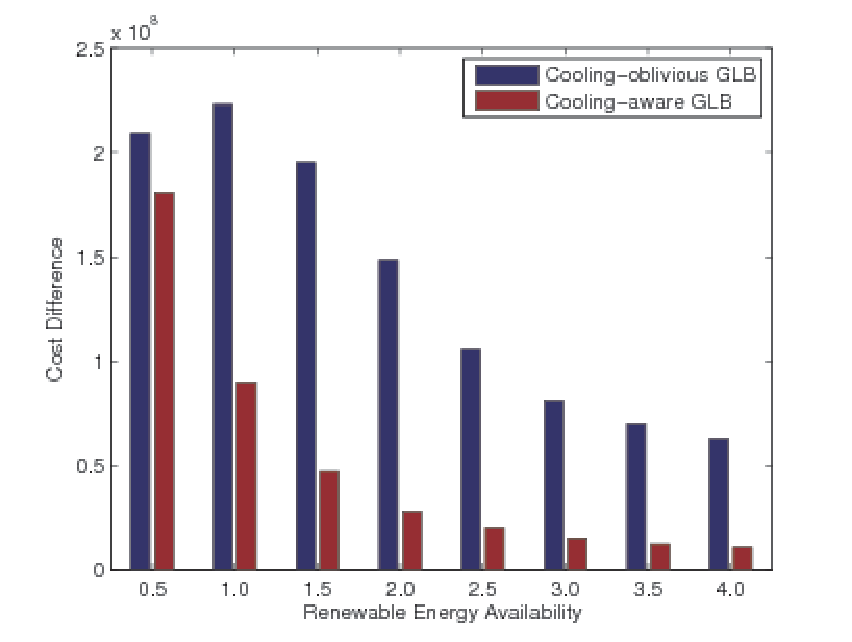
\epsfig{file=cost_diff.pdf, height=2.2in, width=3.2in}
\caption{The difference between optimal costs in summer/winter for both Cooling-aware and Cooling-oblivious GLB}
\end{figure}

The cooling-aware geographical load balancing model reduces firm's energy cost by routing the requests to locations where energy is cheap and cooling is easy. Such savings overweighs the increase in delay cost due to routing. Hence our model matches a profit-maximizing firm's primary interest.  

%In this experiment, the aggregate amount of renewable energy is set to be the total IT demand multiplied by a coefficient, where the coefficient series is the integer multiples of 0.5 within [0.5, 4]. We run the experiment under both summer and winter weather.    

Our first experiment explores the cost savings aspect of the this model. Figure 2 illustrates the extent of total cost savings of our model. We choose the total cost under Cooling-oblivious GLB and LOCAL as the benchmark. The Cooling-aware model has the better cost-saving performance against the benchmarks. This edge is rather clear under two situations. First, in summer when cooling is hard, the Cooling-aware model shows significant improvement even compared to the Cooling-oblivious model; it considers the energy demand for cooling when making routing decisions thus is able to use renewable energy optimally. Second, when the aggregate renewable energy is more than the aggregate demand yet not as much as twice the demand is, some but not all data center locations have surplus in renewables. The Cooling-aware GLB exploits this surplus better than the benchmarks.

We are interested in whether the Cooling-aware GLB model works under all weathers, i.e. how much different the result is when the weather changes. Figure 3 shows the difference between the optimal costs in summer and in winter using each model. The previous Cooling-oblivious model's performance varies significantly with seasonality, whereas our Cooling-aware GLB model's performance is more robust. The result suggests that our Cooling-aware model exploits the heterogeneity in weather to alleviate the energy demand for cooling.    
%\begin{figure}
%\centering
%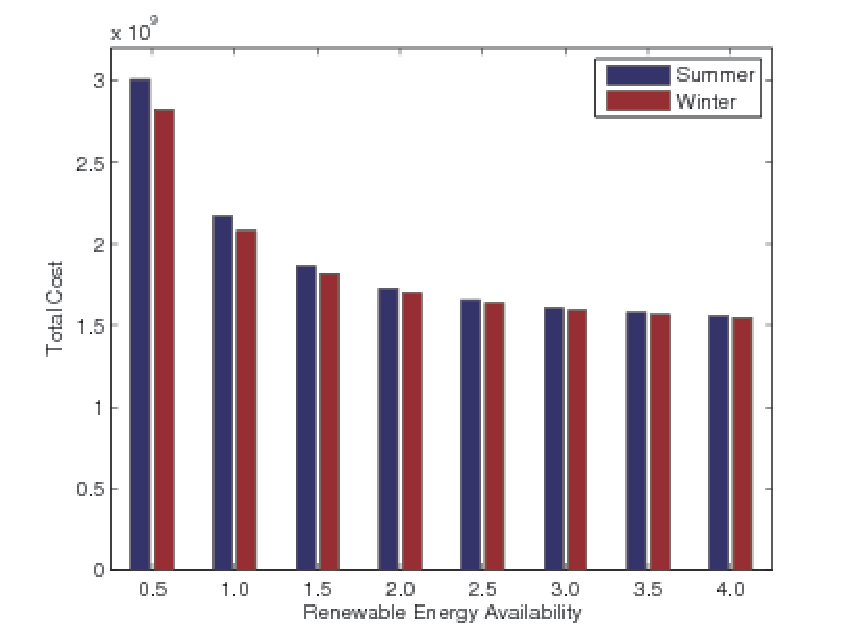
\epsfig{file=opt_cost_comparison.pdf, height=2.2in, width=3.2in}
%\caption{A sample black and white graphic (.eps format).}
%\end{figure}



\subsection{Environmental impact - CO2 savings}


\begin{figure}
\centering
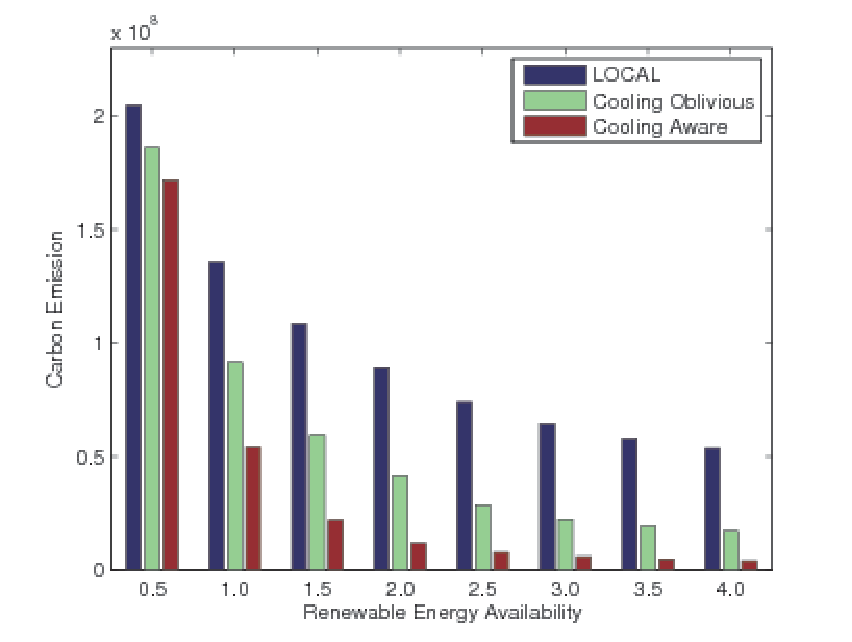
\epsfig{file=carbon_summer.pdf, height=2.2in, width=3.2in}
\caption{Comparison of carbon emission of Cooling-aware CLB, Cooling-oblivious GLB and LOCAL.}
\end{figure}


The geographical load balancing method model benefits from routing requests to where energy price is low. When the data centers have on-site renewable energy plant as in our setting, renewable energy becomes cheap; the model allows optimal usage of these renewables and thus has an desirable side-effect: reducing carbon emission. 

We can quantify the amount of CO2 emission via multiplying the grid energy usage of each data center location by the CO2 emission per energy unit. Figure 4 shows the CO2 emission comparison of each model in summer. By using the Cooling-aware GLB model, the aggregate carbon emission can be reduced by more than 50\% as compared to LOCAL if the total renewable energy supply is equal to the total IT demand. If more renewable energy is available, the carbon emission of Cooling-aware GLB is even less than half of that of Cooling-oblivious GLB. 

The environmental impact of our new model is significant. This result is achieved even when we do not include the benefit of reducing carbon emission in the model. If the firm is given incentives for being environmental friendly, we believe the new model will certainly have more advantage in the cost-saving aspect.



\subsection{GLB versus Storage}

\begin{figure}
\centering
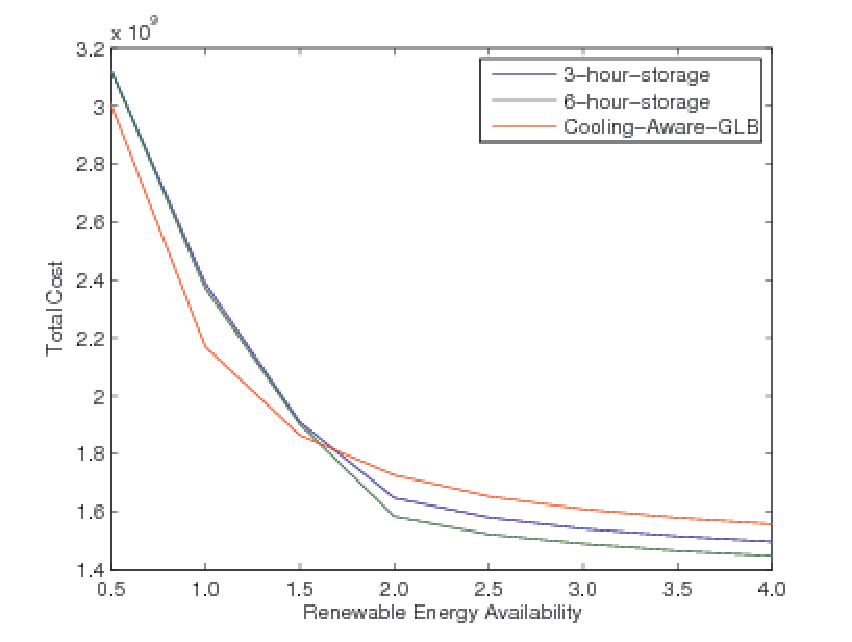
\epsfig{file=cost_storage.pdf, height=2.2in, width=3.2in}
\caption{Comparison of optimal costs of the storage model and the Cooling-aware GLB model.}
\end{figure}
\begin{figure}
\centering
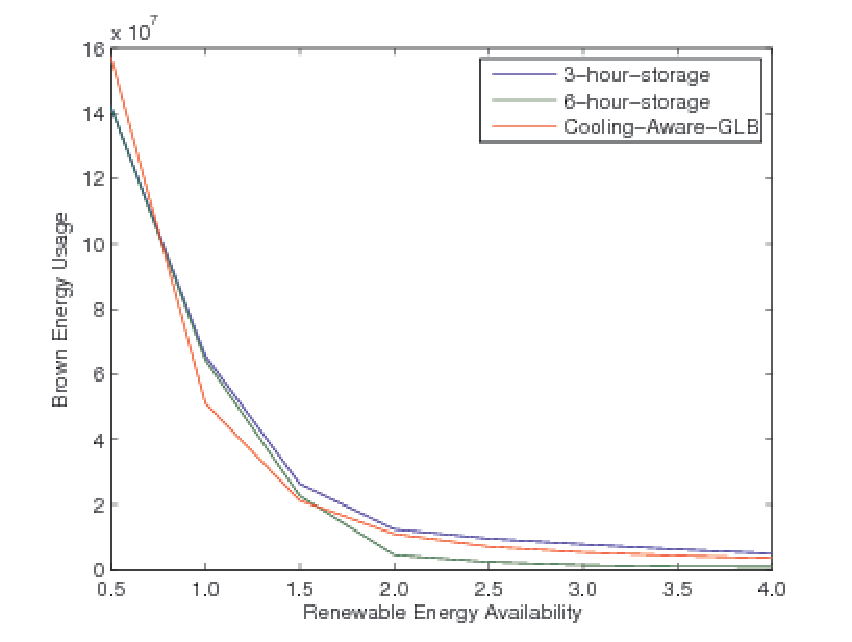
\epsfig{file=brown_storage.pdf, height=2.2in, width=3.2in}
\caption{Comparison of brown energy usage of the storage model and the Cooling-aware GLB model.}
\end{figure}
One alternative way of using renewable energy efficiently is to store the extra renewables at some moments for future use. Unlike the geographical load balancing model which changes the energy demand curve in each location to match the supply, using energy storage reshapes the energy supply curve to fit the demand. We are interested in the characteristics of performance of both methods. In this experiment, we compare the cost curve and the brown energy usage curve of using GLB and using storage. Since our experiment starts at midnight, the time when the data centers are likely to have used all of its storage for batch jobs \cite{adam:cooling}, we assume that the storage starts empty. 

Figure 5 illustrates the trend of optimal costs of these models with respect to varying renewable availability. We notice that the Cooling-aware GLB has cost advantage when the total renewable energy is less than 1.5 times of the aggregate IT demand. The storage model, on the other hand, has cost advantage when the renewable energy supply is in large surplus. 

Figure 6 shows the comparison of brown energy usage of each model. The result suggests that the Cooling-aware GLB model needs less energy from the grid compared to the 6-hour-storage curve when the total renewable supply is less than 1.5 times of the total IT power demand. Moreover, it needs less grid energy than the total renewable energy compared to the 3-hour-storage model in almost the entire renewable availability interval except when the renewable availability coefficient is 0.5. The environmental impact advantage of our new model is even more significant compared to the cost advantage.  

We thus can conclude that our model is better than the storage model when the renewable generation facilities are not saturatedly established yet; it requires less prior investment on infrastructures.

\bibliographystyle{abbrv}
\bibliography{surfReport}
\end{document}
